
\documentclass{article}
\usepackage{graphicx,wrapfig,lipsum}

\usepackage{tikz}

%------------------------------------------
\begin{document}


\begin{wrapfigure}{r}{0.28\textwidth}
	%\caption{A Thionyl Chloride Question in XpdfReader}
\label{fig:tc}
\begin{tikzpicture}

\node[inner sep=0pt] (x1) at (0,0)
    {\includegraphics[width=110mm, 
    	trim={104mm 10mm 1mm 34mm},clip]
    	{xScreenShot2.png}};

\curicon{0.89}{-2.16}

\rectann{darkRed!50}{0.7}{2pt}{logoCyan}{0.5}{-1.3,-2.41}{6.45}{3.1}{1.1}

\end{tikzpicture}


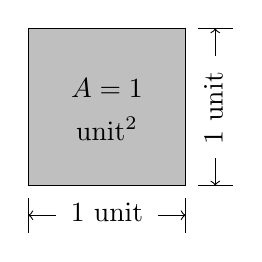
\begin{tikzpicture}
	\draw [fill = lightgray] rectangle (2,2);
	\node [right, rotate=90] at (2.35,0.4) {1 unit};
	\node [below] at (1,-0.1) {1 unit};
	\node [above] at (1,1) {$A = 1$};
	\node [below] at (1,1) {$\textrm{unit}^2$};
	\draw [<-] (0,-0.375) -- (0.35,-0.375);
	\draw [->] (1.65,-0.375) -- (2,-0.375);
	\draw (0,-0.15) -- (0,-0.6);
	\draw (2,-0.15) -- (2,-0.6);
	\draw [<-](2.375,0) -- (2.375,0.35);
	\draw [->](2.375,1.65) -- (2.375,2);
	\draw (2.15,0) -- (2.6,0);
	\draw (2.15,2) -- (2.6,2);
\end{tikzpicture}
	%\caption{Launching IQmol from a practice test question.}
	%\label{f:diagram}


\end{wrapfigure}

\lipsum[2-3]
\end{document}
